\section{Model}
In order to reliably reproduce experimental observations of dynein's stepping, a model of dynein should responsibly conserve dynein's spatial information and complex structure under an aqueous environment. Doing so computationally introduces a strict balance between model accuracy and computational efficiency. In an attempt to best satisfy this difficult balance, we propose a coarse-grained model of dynein under a series of assumptions that benefits quick simulations of dynein taking a step. 


\subsection{2D Rigid Rod Model}
Since our goal is to investigate dynein's inter-step correlation during its forward directed stepping, we decided to model dynein as a 2-dimensional system of circular domains held together by massless rigid rods. These domains entitle two binding domains, two motor domains, and one tail domain, where each domain act as independent angular springs with their own spring constants.

\begin{figure}[H]
	\centering
	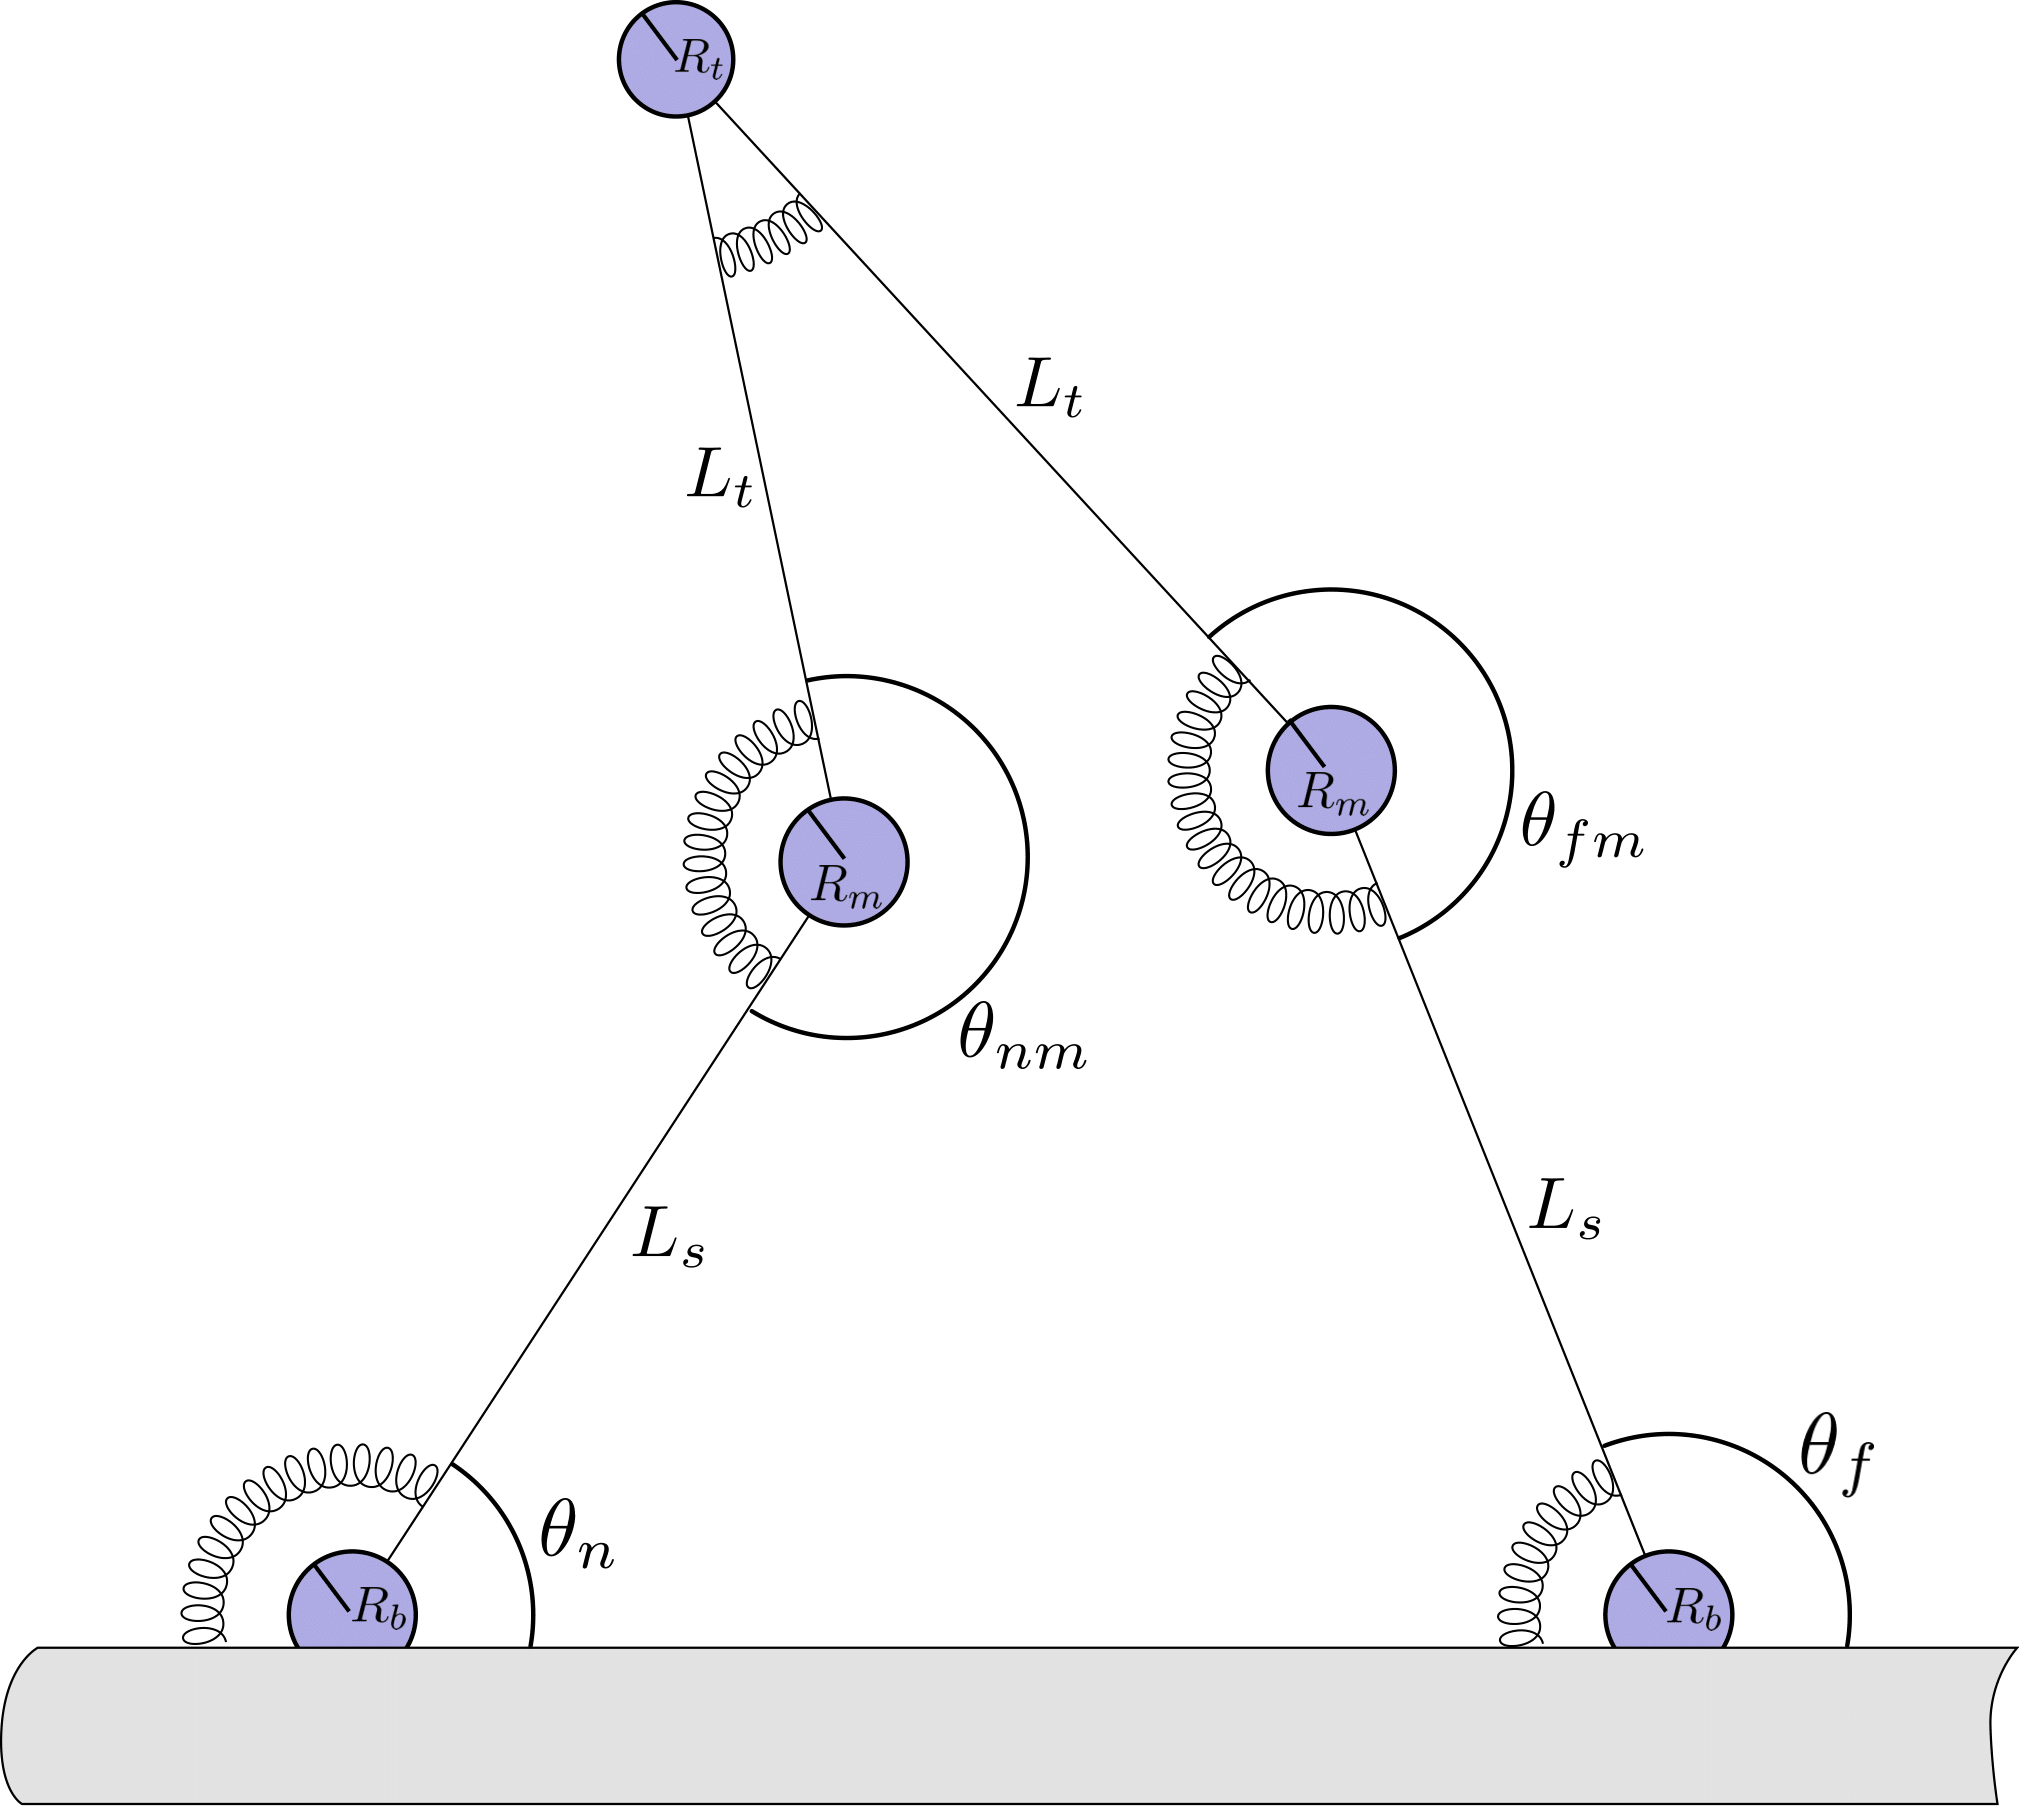
\includegraphics[width=0.6\columnwidth]{Figures/model-cartoon.png}
	\caption[Dynein Model]{\textbf{Dynein Model} \cite{Capek2017}}
	\label{fig:model}
\end{figure}

Despite dynein's complexity allowing its step to vary in both length and direction, we limit our model to one direction to eliminate a dimension (the off-axis) when analyzing the forward stepping pattern of dynein. This would also simplify the asymmetry of the microtubule when the dynein is stepping either on the $\alpha$ or $\beta$ tubulin. We also simplify the stalk and linker to be massless because we are assuming the drag force to be much larger than the mass of the rods and domains. The reasoning for this will be later discussed in Section \hyperref[sec:BrownianDynamics]{3.3} when we introduce Brownian dynamics. Although the stalk and linker of real dynein definitely have mass, we counteract the loss of interactions the rods experience with its environment by increasing the radii of the domains to be slightly larger than experimental measurements.

\subsection{Domains as Angular Springs}
In order to best simulate the stretching and forward kicking motion of the power stroke, we defined our domains to act as springs with spring constants $c_b$, $c_m$, and $c_t$ -- one for each respective domain. This can be analogous to how humans walk using their knees and ankles to bend and stretch accordingly when taking a step. Defining our domains as springs will allow us to influence forward bias walking by introducing a restoring force in each domain using Hooke's law: 
\begin{equation}
    F_i=-c_i(\theta_i-\theta_{i,eq})
\end{equation}
where $c_i$ is the spring constant, $\theta_i$ is angle corresponding to the $i^{th}$ domain, and $\theta_{i,eq}$ is the equilibrium angle in which biases the motion. Using this, we can calculate the energy of each domain by integrating and arriving to the familiar equation for spring energy.
\begin{equation}
    U_i=\frac{1}{2}c_i(\theta_i-\theta_{i,eq})
\end{equation}
Since dynein is symmetric for each heavy chain leg, the equilibrium angle will be identical for both binding and motor domain pairs, i.e. $\theta_{b,eq}$ is defined as the equilibrium angle for both binding domains, while $\theta_{m,eq}$ is defined as the equilibrium angle for both motor domains. This equation would then be used throughout the entirety of the simulation to determine the total energy of our dynein at a given conformation. 


\subsection{Two-State System}
According to the Mechanochemical Cycle (\hyperref[fig:MechanochemicalCycle]{Figure 2.5}), dynein can be in eight states over the course of a single step. However, many of these states possess similar conformations, where the dynein has either one binding domain bounded with the other diffusing above the microtubule or both binding domains bounded. Since the states that take the most time are during binding and unbinding \cite{}, we categorized the cycle into two main conformations: the pre-stroke one bound state and the post-stroke both bound state.

\begin{figure}[H]
	\centering
	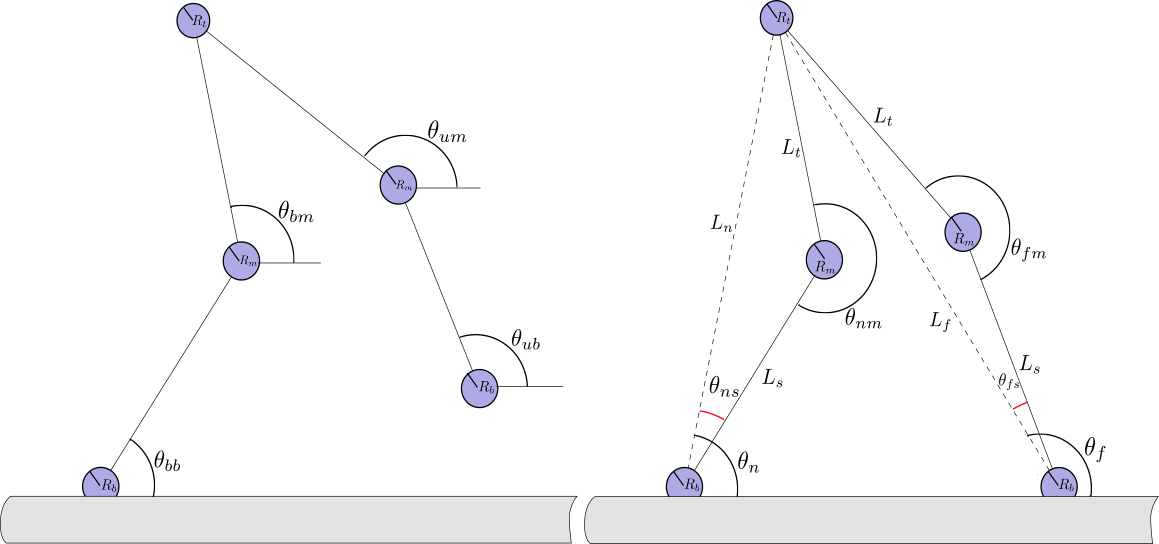
\includegraphics[width=0.8\columnwidth]{Figures/OB_vs_BB.PNG}
	\caption[One Bound vs. Both Bound]{\textbf{One Bound vs. Both Bound} Figure on left: Prestroke one bound state with labeling scheme ‘bounded’ and ‘unbouded’ for bounded leg and unbounded leg. Figure on the right: Poststroke both bound state with labeling scheme ‘near’ and ‘far’ for identifying heavy chain subunits \cite{Capek2017}.}
	\label{fig:final_disp}
\end{figure}

Differentiating the two allows us to more conveniently bias the conformational change by defining different equilibrium angles for both states.  


\subsection{Transitioning Between States}
\textit{Physics about conformational energy changes. How we model transitioning between BB state and OB state using transitioning rates and spring energies.}


\section{Simulation}
\textit{Pulled from Methods section. Maybe add a little intro to simulation process}
\par
These quick simulations are governed by a Monte Carlo algorithm, while the movement of the model is dictated by equations of motion describing domains interacting with a force of drag and a random force. This type of molecular simulations are more commonly known as Brownian dynamics. (\textbf{Possible take out sentence introducing MC and Brownian dynamics for later})


\subsection{Monte Carlo Algorithm}
\textit{Physics background on Monte Carlo. Stat Mech. }


\subsection{Brownian Dynamics}
\label{sec:BrownianDynamics}
\textit{Physics background on Brownian dynemaics. Newton's second law. What forces will we use? How do we determine the random force? etc.}

\subsection{Equations of Motion}
\textit{Derived equations of motion for each domain of our dynein from Brownian dynamics.}


\textit{STRAIGHT FROM PROPOSAL. FIXME}


Our entire model of dynein will be coded with a combination of both Python and C++. The structural features of dynein will be captured with a two-dimensional geometric model of circular domains connected by rigid rods. The dynamics of dynein will be captured by imposing both equilibrium and Brownian forces on each circular domain of the model, while the chemical properties will be modeled by sporadically transitioning between two states: a poststroke both bound state, and a prestroke one bound state. These two states are shown below in Figure 2.

The simulation for stepping will consist of running multiple independent steps that starts in a both bound configuration and transitions into the Brownian dynamics one bound state. In this state, each domain will undergo Brownian forces until the unbounded leg diffuses back onto the microtubule, thus completing a step. The Brownian dynamics only affects the one bound state since that is the only time (in our model) the domains undergo molecular interaction with its surroundings to achieve processive motion. This Monte Carlo method of collecting an ensemble of statistics after many simulations will lead to probability distributions of measured variables that can be compared with experimental results. The common experimental results analyzed in this field are the distribution of step lengths (defined as the final displacement of the “stepping” leg minus the initial displacement), stepping times, probability of the binding domain unbinding, and the velocity of a step. Once sufficient data is collected for each listed variable, plotting scripts on Python will be used to visualize the possible relationships between these variables and generate analysis for our model’s stepping patterns. Currently, a paper published by Dr. Ahmet Yildiz from the University of Berkeley proposed a possible relationship within dynein’s stepping, implying inter-step correlation [3]. Our model aims to reproduce these results by finding a set of parameters that matches Yildiz’s observation in the form of a linear regression of the step lengths against the initial binding domain separation. We hope to either support Yildiz’s claim or infer some new property of dynein that generated Yildiz’s observation.